%%%%%%%%%%%%%%%%%%%%%%%%%%%%%%%%%%%%%%%%%%%%%%%%
%% Intro to LaTeX and Template for Homework Assignments
%% Quantitative Methods in Political Science
%% University of Mannheim
%% Fall 2019
%%%%%%%%%%%%%%%%%%%%%%%%%%%%%%%%%%%%%%%%%%%%%%%%

% created by Marcel Neunhoeffer & Sebastian Sternberg


% This template and tutorial will help you to write up your homework. It will also help you to use Latex for other assignments than this course's homework.

%%%%%%%%%%%%%%%%%%%%%%%%%%%%%%%%%%%%%%%%%%%%%%%%
% Before we get started
%%%%%%%%%%%%%%%%%%%%%%%%%%%%%%%%%%%%%%%%%%%%%%%%

% Make an account on overleaf.com and get started. No need to install anything.

%%%%%%%%%%%%%%%%%%%%%%%%%%%%%%%%%%%%%%%%%%%%%%%%
% Or if you want it the nerdy way...
% INSTALL LATEX: Before we can get started you need to install LaTeX on your computer.
				% Windows: http://miktex.org/download
				% Mac:         http://www.tug.org/mactex/mactex-download.html	
				% There a many more different LaTeX editors out there for both operating systems. I use TeXworks because it looks the same on Windows and Mac.
				

% SAVE THE FILE: The first thing you need to do is to save your LaTeX file in a directory as a .tex file. You will not be able to do anything else unless your file is saved. I suggest to save the .tex file in the same folder with your .R script and where you will save your plots from R to. Let's call this file template_homework1.tex and save it in your Week 1 folder.


% COMPILE THE FILE: After setting up your file, using your LaTeX editor (texmaker, texshop), you can compile your document using PDFLaTeX.
	% Compiling your file tells LaTeX to take the code you have written and create a pdf file
	% After compiling your file, in your directory will appear four new files, including a .pdf file. This is your output document.
	% It is good to compile your file regularly so that you can see how your code is translating into your document.
	
	
% ERRORS: If you get an error message, something is wrong in your code. Fix errors before they pile up!
	% As with error messages in R, google the exact error message if you have a question!
%%%%%%%%%%%%%%%%%%%%%%%%%%%%%%%%%%%%%%%%%%%%%%%%


% Now again for everyone...

% COMMANDS: 
	% To do anything in LaTeX, you must use commands
	% Commands tell LaTeX when to start your document, how you want your document to look, and how to format your document
	% Commands ALWAYS begin with a backslash \

% Everything following the % sign is a comment and will not be used by Latex to compile your document.
% This is very similar to # comments in R.

% Every .tex file usually consists of four parts.
% 1. Document Class
% 2. Packages
% 3. Header
% 4. Your Document

%%%%%%%%%%%%%%%%%%%%%%%%%%%%%%%%%%%%%%%%%%%%%%%%
% 1. Document Class
%%%%%%%%%%%%%%%%%%%%%%%%%%%%%%%%%%%%%%%%%%%%%%%%
 
 % The first command you will always have will declare your document class. This tells LaTeX what type of document you are creating (article, presentation, poster, etc). 
% \documentclass is the command
% in {} you specify the type of document
% in [] you define additional parameters
 
\documentclass[a4paper,11pt]{article} % This defines the style of your paper

% We usually use the article type. The additional parameters are the format of the paper you want to print it on and the standard font size. For us this is a4paper and 12pt.

%%%%%%%%%%%%%%%%%%%%%%%%%%%%%%%%%%%%%%%%%%%%%%%%
% 2. Packages
%%%%%%%%%%%%%%%%%%%%%%%%%%%%%%%%%%%%%%%%%%%%%%%%

% Packages are libraries of commands that LaTeX can call when compiling the document. With the specialized commands you can customize the formatting of your document.
% If the packages we call are not installed yet, TeXworks will ask you to install the necessary packages while compiling.

% First, we usually want to set the margins of our document. For this we use the package geometry. We call the package with the \usepackage command. The package goes in the {}, the parameters again go into the [].
\usepackage[top = 2.5cm, bottom = 2.5cm, left = 2.5cm, right = 2.5cm]{geometry} 

% Unfortunately, LaTeX has a hard time interpreting German Umlaute. The following two lines and packages should help. If it doesn't work for you please let me know.
\usepackage[T1]{fontenc}
\usepackage[utf8]{inputenc}

% The following two packages - multirow and booktabs - are needed to create nice looking tables.
\usepackage{multirow} % Multirow is for tables with multiple rows within one cell.
\usepackage{booktabs} % For even nicer tables.

% As we usually want to include some plots (.pdf files) we need a package for that.
\usepackage{graphicx} 

% The default setting of LaTeX is to indent new paragraphs. This is useful for articles. But not really nice for homework problem sets. The following command sets the indent to 0.
\usepackage{setspace}
\setlength{\parindent}{0in}

% Package to place figures where you want them.
\usepackage{float}

% Package for figures and subfigures
\usepackage{caption}
\usepackage{subcaption}

% Wrap text around figures
\usepackage{wrapfig}

% The fancyhdr package let's us create nice headers.
\usepackage{fancyhdr}

% Import ams math backages
\usepackage{amsmath}
\usepackage{amssymb}
\usepackage{amsfonts}
\usepackage{bbm}
\usepackage{lstbayes}
\usepackage{bm}

% Referencing
\usepackage{biblatex}
\addbibresource{../reference_material/references.bib}

% For csv file display
\usepackage[l3]{csvsimple}

% Listings
\usepackage{listings}
\usepackage{xcolor}
\usepackage{xparse}

\NewDocumentCommand{\codeword}{v}{%
\texttt{\textcolor{blue}{#1}}%
}

% Arrays from csv 
\usepackage{pgfplotstable}
\usepackage{array}

\pgfplotsset{
    /pgfplots/table/omit header/.style={%
        /pgfplots/table/typeset cell/.append code={%
            \ifnum\c@pgfplotstable@rowindex=-1
                \pgfkeyslet{/pgfplots/table/@cell content}\pgfutil@empty%
            \fi
        }
    }
}

\definecolor{codegreen}{rgb}{0,0.6,0}
\definecolor{codegray}{rgb}{0.5,0.5,0.5}
\definecolor{codepurple}{rgb}{0.58,0,0.82}
\definecolor{backcolour}{rgb}{0.95,0.95,0.92}

\lstdefinestyle{mystyle}{
    backgroundcolor=\color{backcolour},   
    commentstyle=\color{codegreen},
    keywordstyle=\color{magenta},
    numberstyle=\tiny\color{codegray},
    stringstyle=\color{codepurple},
    basicstyle=\ttfamily\footnotesize,
    breakatwhitespace=false,         
    breaklines=true,                 
    captionpos=b,                    
    keepspaces=true,                 
    numbers=left,                    
    numbersep=5pt,                  
    showspaces=false,                
    showstringspaces=false,
    showtabs=false,                  
    tabsize=2
}

\lstset{style=mystyle}

% Tiks for drawing graphs
\usepackage{tikz}
\usetikzlibrary{positioning}

% For drawing text boxes
\usepackage[many]{tcolorbox}

\newtcolorbox{boxA}{
    fontupper = \bf,
    boxrule = 1.5pt,
    colframe = black % frame color
}


% Blind text
\usepackage{blindtext}

%%%%%%%%%%%%%%%%%%%%%%%%%%%%%%%%%%%%%%%%%%%%%%%%
% 3. Header (and Footer)
%%%%%%%%%%%%%%%%%%%%%%%%%%%%%%%%%%%%%%%%%%%%%%%%

% To make our document nice we want a header and number the pages in the footer.

\pagestyle{fancy} % With this command we can customize the header style.

\fancyhf{} % This makes sure we do not have other information in our header or footer.

\lhead{\footnotesize UDA: Final Project}% \lhead puts text in the top left corner. \footnotesize sets our font to a smaller size.

%\rhead works just like \lhead (you can also use \chead)
\rhead{\footnotesize CCID: 00951537} %<---- Fill in your lastnames.

% Similar commands work for the footer (\lfoot, \cfoot and \rfoot).
% We want to put our page number in the center.
\cfoot{\footnotesize \thepage} 


%%%%%%%%%%%%%%%%%%%%%%%%%%%%%%%%%%%%%%%%%%%%%%%%
% 4. Your document
%%%%%%%%%%%%%%%%%%%%%%%%%%%%%%%%%%%%%%%%%%%%%%%%

% Now, you need to tell LaTeX where your document starts. We do this with the \begin{document} command.
% Like brackets every \begin{} command needs a corresponding \end{} command. We come back to this later.

\usepackage{hyperref}
\hypersetup{
    colorlinks=true,
    linkcolor=blue,
    filecolor=magenta,      
    urlcolor=cyan,
    pdftitle={Overleaf Example},
    pdfpagemode=FullScreen,
    }

\begin{document}


%%%%%%%%%%%%%%%%%%%%%%%%%%%%%%%%%%%%%%%%%%%%%%%%
%%%%%%%%%%%%%%%%%%%%%%%%%%%%%%%%%%%%%%%%%%%%%%%%

%%%%%%%%%%%%%%%%%%%%%%%%%%%%%%%%%%%%%%%%%%%%%%%%
% Title section of the document
%%%%%%%%%%%%%%%%%%%%%%%%%%%%%%%%%%%%%%%%%%%%%%%%

% For the title section we want to reproduce the title section of the Problem Set and add your names.

\thispagestyle{empty} % This command disables the header on the first page. 

\begin{tabular}{p{15.5cm}} % This is a simple tabular environment to align your text nicely 
{\large \bf MATH70103: Unstructured Data Analysis} \\
Imperial College London \\ Autumn 2023  \\ CCID: 00951537\\
\hline % \hline produces horizontal lines.
\\
\end{tabular} % Our tabular environment ends here.

\vspace*{0.3cm} % Now we want to add some vertical space in between the line and our title.

\begin{center} % Everything within the center environment is centered.
	{\Large \bf Final Project} % <---- Don't forget to put in the right number	
\end{center}  

\vspace{0.4cm}

%%%%%%%%%%%%%%%%%%%%%%%%%%%%%%%%%%%%%%%%%%%%%%%%
%%%%%%%%%%%%%%%%%%%%%%%%%%%%%%%%%%%%%%%%%%%%%%%%

\textbf{Plagiarism Statement}: \emph{The following assignment is a product of my own work.}

\medskip

%% Abstract Here
\subsection*{Abstract}

In this report I explore the effectiveness of Convolutional Neural Networks in identifying images
that contain fires in the wild, with the aim of producing an algorithm that could potentially be incorporated 
in early wildfire detection systems. I make use of the FLAME (Fire Luminoscity Airbourne-based Machine learning Evaluation)
dataset \cite{FLAME_dataset} and build upon the \emph{Xception} Deep Convolutional Neural network proposed by Google \cite{Xception,Szegedy_2016_CVPR,Szegedy_Ioffe_Vanhoucke_Alemi_2017}.
Key metrics such as binary accuracy, precision and recall are presented for training, validation, testing, and out of sample testing, the latter
of which examines the performance of the model on images outside of the \emph{FLAME} dataset. For this purpose, I use the Fire Classification dataset
available on Kaggle \cite{Kaggle_FIRE_Dataset}.

\medskip

All code and a 100MB subset of the FLAME Dataset have been uploaded to the following Github Repositry: \citeurl{Batek_Unstructured_Data_Analysis}

\tableofcontents

\section{Introduction and Problem Statement}

Wildfires are a pervasive issue across the globe today, causing millions of dollars in damage every year, loss
in natuaral biodiversity in the affected areas, and significant loss and trauma to the affected communities. Recent examples of significant
wildfires include the 2023 Canadian wildfire season \cite*{Milman_2023}, the 2019-20 Australian bushfires (nicknamed ``The Black Summer'') \cite{Aus_bushfires},
and the fires in my home town of Cape Town this Christmas season \cite{Cape_Fires}. It is widely known that natural occuring fires are an integral
part of many ecosystems, as they clear out dead organic matter that prevents living orgnisms from accessing vital nutrients \cite{fire_benefits}, alongside numerous other benefits \cite{bond2017fires}. 
However multiple sources cite an increasing rate of occurence and degree of severity of global wildfires, past the point of biological sustainability \cite{}. This phenomenan is widely attributed
to human intervention such as ... .

The above justifies the need to develop novel methods for detecting wildfires, so that we may anticipate and manage the impact of wildfires in the best way possible. Upon reviewing multiple early-wildfires detection systems,
\Citeauthor{UAV_Wildfire} found that the combined used of unmanned aerial vehicles (UAVs), mounted high resolution imagery and Deep Learning techniques provided the most promising
results in terms navigability, versitility, speed and accuracy. \Citeauthor{FLAME_dataset} introduce a high-resulution image dataset composed of drone footage frames that were taken during a perscribed burning
slash piles in Northern Arizona. In that same paper, the Google-Keras \emph{Xception} network was applied to create a binary classifier model for fire image detection. 

The problem statement for this report is therefore as follows:

\begin{boxA}
    \underline{Problem Statement:}
\begin{itemize}
    \item Train a Convolutional Neural Network classifier for fire image classification.
    \item Investigate the effect of the preprocessing, hidden and output layers of the trained CNN model on an example image.
    \item Evaluate the Accuracy, Precision and Recall of the model on Validation, Testing and Out-of-Sample images.
\end{itemize}
\end{boxA}


\section{Image Dataset}

\subsection{Data Selection}
%% Introduce the criteria by which the datasets were chosen
Multiple datasets were considered for the purposes of this report, from sources such as Kaggle, and other publicaly available portals. Besides the stated
criteria for this project (complexity and originality), I also aimed to use a dataset that is suitable given the findings in \citetitle{UAV_Wildfire}, wherein \Citeauthor{UAV_Wildfire} argue that UAV-sensor
technology is more suitable for autonomous fire detection systems in terms of cost, accuracy and practicality than alternatives such as satellite imagery or stationery platforms.
The ideal dataset would therefore include images taken from the perspective of UAVs.

\medskip

To this end the FLAME Dataset produced by \Citeauthor{FLAME_dataset} addresses these criteria explicitly. The dataset includes drone imagery taken of the perscribed burning
of slash piles in the forests of Arizona during January 2020, during which time the weather conditions were generally cloudy with an average temparature of -6 $^{\circ}$C. The following Exploratory Data Anylisis includes visualizations of a few example images in the dataset.
The full published dataset includes video footage, images, a variety of specturms used (including the normal RGB, fusion, white-hot and green-hot palettes), as well as images and masks for fire image segmentation (identifying the fire pixels in an image, thereby identifying where
the fire is situated from the perspective of the UAV). For the purposes of this report, I use only the \textbf{Training, Validation and Test} classifiction images (all in the normal RGB spectrum), namely items 7) and 8)
in the following IEEE-Dataport link: \url{https://ieee-dataport.org/open-access/flame-dataset-aerial-imagery-pile-burn-detection-using-drones-uavs}.

\medskip

The classification dataset above is 1.46 GB in size. For the purpose of submission, I have produced a 100MB subset of this dataset using random sampling, and uploaded it to the the aforementioned Github repository, under \verb!data/FLAME_dataset_subset!. However,
note that the model and results described in the following report were compiled on the basis of the entire set of images.

\subsection{Exploratory Data Analysis}
In this section, I aim to visualise the data downloaded from points 7) and 8) on the aforementioned IEEE-Dataport. As a first step, I visualise the directory
heirarchy structure in \verb!scripts/UDA_FinalProject_Batek.ipynb!:

\begin{figure}[h]
    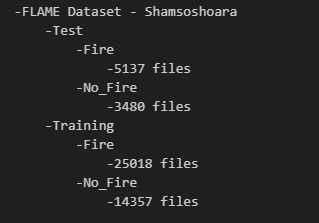
\includegraphics{../figures/FLAME_dataset_structure.png}
    \caption{File structure of the Classification images in the FLAME Dataset}
\end{figure}

Figure 1 shows that the dataset contains 47992 images, 8617 (18\%) of which are in
the test set with the remaining 82\% in the training\//validation set. Examining the file counts clearly shows that there is a significant class imbalance 
between Fire and Non-Fire images, and that the Fire Class is overrepresented in the training set relative to the Test set. This imabalance will likely
influence model specificity and recall later on.

\medskip

As a next step, I investigate the image dimensions and the pixel values in the training set:

\begin{figure}[h]
    \centering
    \begin{subfigure}[b]{0.45\textwidth}
        \centering
        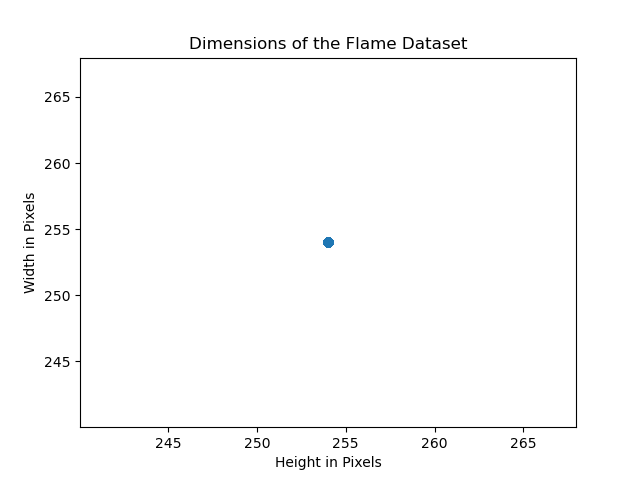
\includegraphics[width=\textwidth]{../figures/flame_dataset_image_dimensions.png}
    \end{subfigure}
    \hfill
    \begin{subfigure}[b]{0.45\textwidth}
        \centering 
        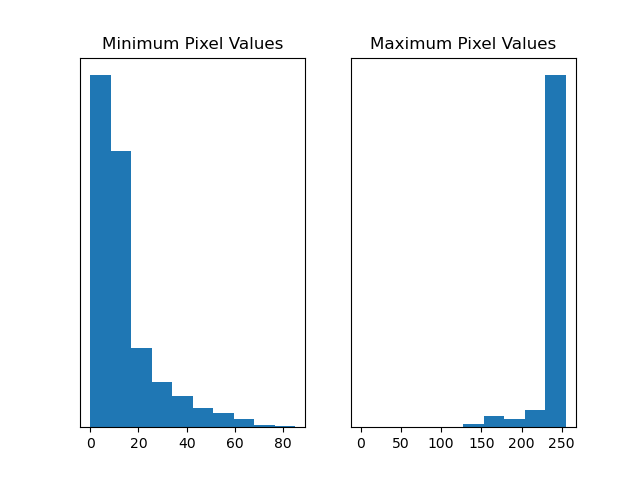
\includegraphics[width=\textwidth]{../figures/pixel_ranges.png}
    \end{subfigure}
    \caption{Training set image dimensions in pixels (left), and distribution of minimum and maximum pixel values (right).}
\end{figure}

It is shown in Figure 2 above that all of the images in the dataset have been rescaled to 254x254 pixels (left), whereas the pixel
ranges vary between 0 to 255 (right). This is taken account of in the preprocessing layers of the CNN model later on.

\medskip

As a final step in the Exploratory Data Analysis, I randomly choose 1 image for each set\//class combination
and display them:

\begin{figure}[h]
    \centering
    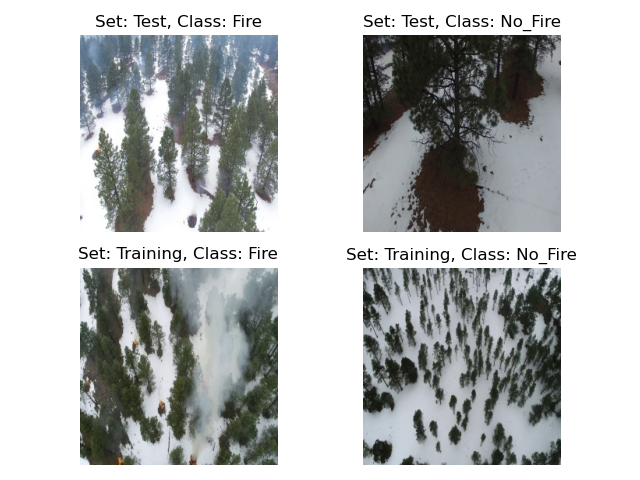
\includegraphics{../figures/example_images.png}
    \caption{Four images from the FLAME dataset}
\end{figure}

The images in Figure 3 appear as expected given that they were taken in Arizona in the winter month of January.
The weather at the time was generally cloudy, and despite the fact that most of the images do not show any portion of
the sky (the drone mounted cameras tend to be pointed at the ground), the affect of the weather on the lighting is apparent
in the images. The ground in the images tends to be covered in snow, with the crucial exceptions of the fires and under the trees.
This all raises the question as to whether a CNN model trained on these images would perform equally well in identifying fires in images
taken in different environments and weather conditions (such as during the summer, when the risk of wildfires is the highest). It is for this
purpose that I evaluate the CNN model against out of sample images later on in the report.



\section{Analysis}
In this section, I will introduce and justify the use of the Convolutional Neural Network architecture that I have chosen when training the
classifier model for image fire detection. This is a simplified version of the Google-Keras Xception network adopted by \Citeauthor*{FLAME_dataset} in \citetitle{FLAME_dataset}. I will also discuss the model's accuracy, precision, recall and AUC statistics during training, validation and testing against 
unseen in-sample and out-of-sample images.

\subsection{The Google-Keras Xception Network}
The Xception Network is a deep Convolutional Neural Network (DCNN) developed by Google researchers \Citeauthor{Xception} \cite{Xception} and \Citeauthor{Szegedy_2016_CVPR} \cite{Szegedy_2016_CVPR,Szegedy_Ioffe_Vanhoucke_Alemi_2017}.
It builds upon previous the previous Inception architecture by replacing the Inception modules therein with depth-wise separable convolutions.

\pagebreak

\begin{wrapfigure}{l}{0.45\textwidth}
    \begin{center}
        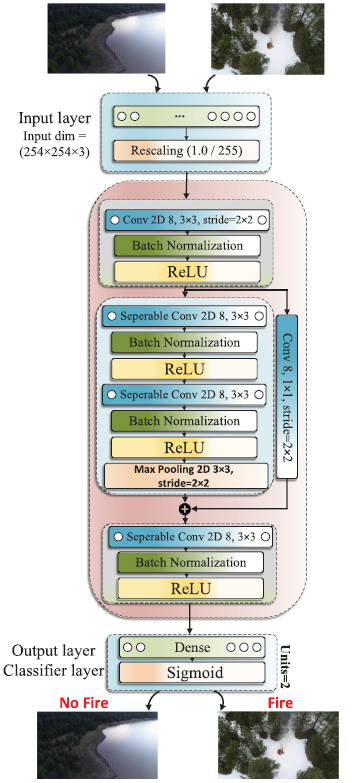
\includegraphics[width=0.43\textwidth]{../figures/Xception_network.png}
    \end{center}
    \caption{Xception Network graph, as used in \cite{FLAME_dataset}}
\end{wrapfigure}

For the perposes of this report, I make use of and build upon a simplified version of the Xception framework used in \cite{FLAME_dataset}, which is visualized
in Figure 4. The network can be subdivided into input (top - blue), hidden (middle - red) and output (bottom - blue) blocks. The input block for the model used in \cite{FLAME_dataset}
initially only included an input and a Rescaling layer for mappping the integer 0-255 range pixel values to float 0-1 values. I further incorporated a Random Data Augmentation
layer (a layer sequentially containing Random Flip and Random rotation layers) in order to introduce some variability to the input data during training, so as to reduce model overfitting
and improve general applicability. This was particularly necessary in the case of the FLAME dataset, which is comprised of video footage frames, and therefore has a high degree of internal similarity.
(In plan language, two frames near the same point in a video are going to materialy look the same).

\medskip

The hidden block is comprised of several depth-wise separable convolutions, and a shortcut layer between the first and last convolution blocks. The first set of layers in the hidden block
contains a 2 dimensional convolutional layer with 8 output channels, a 3x3 kernal and a stride of 2. The remainder if the hidden block contains separable 2D convolutional layers with similar settings.
Each convolution block includes a Batch Normalization layer as well as a Rectified Linear Unit activation layer. The prior speeds up the training process by and reduces the likelihood of overfitting by
decreasing the importance of the initial model weights, wheres the latter floors the pixel values to zero.

\medskip

Finally, the output layer summarizes the average pixel values in the 8 channels outputted from the hidden block into a single vector in $\mathbb{R}^8$, $\vec{x}$. For the purpose of binary classification,
this is then converted to a probability score by use of the \emph{Sigmoid function}:

\[
    P(\text{label}=\text{fire}) = \frac{1}{1 + e^{-\vec{\beta} \cdot \vec{x}}}
\] 

where $\vec{\beta}$ is the weight vector for the last layer in the network. 

Figure 5 demonstrates the result of each distinct block in the model. Firstly, 
we see how the input layer augments the original input image by randomly flipping and rotating
it. We then see how each convolution block (2D convolution, batchnormalization and ReLU activation)
incrementally segments the image, and places emphases on the pixels that contain the fire. The Global
Average Pooling layer then summarizes the average pixel values per channel, wherein the
channels that emphasis the fire more directly have a higher score. Finally, the Global Average
Pooling vector is passed through the Sigmoid function to produce a final probability score for the
image.

\begin{figure}
    \centering
    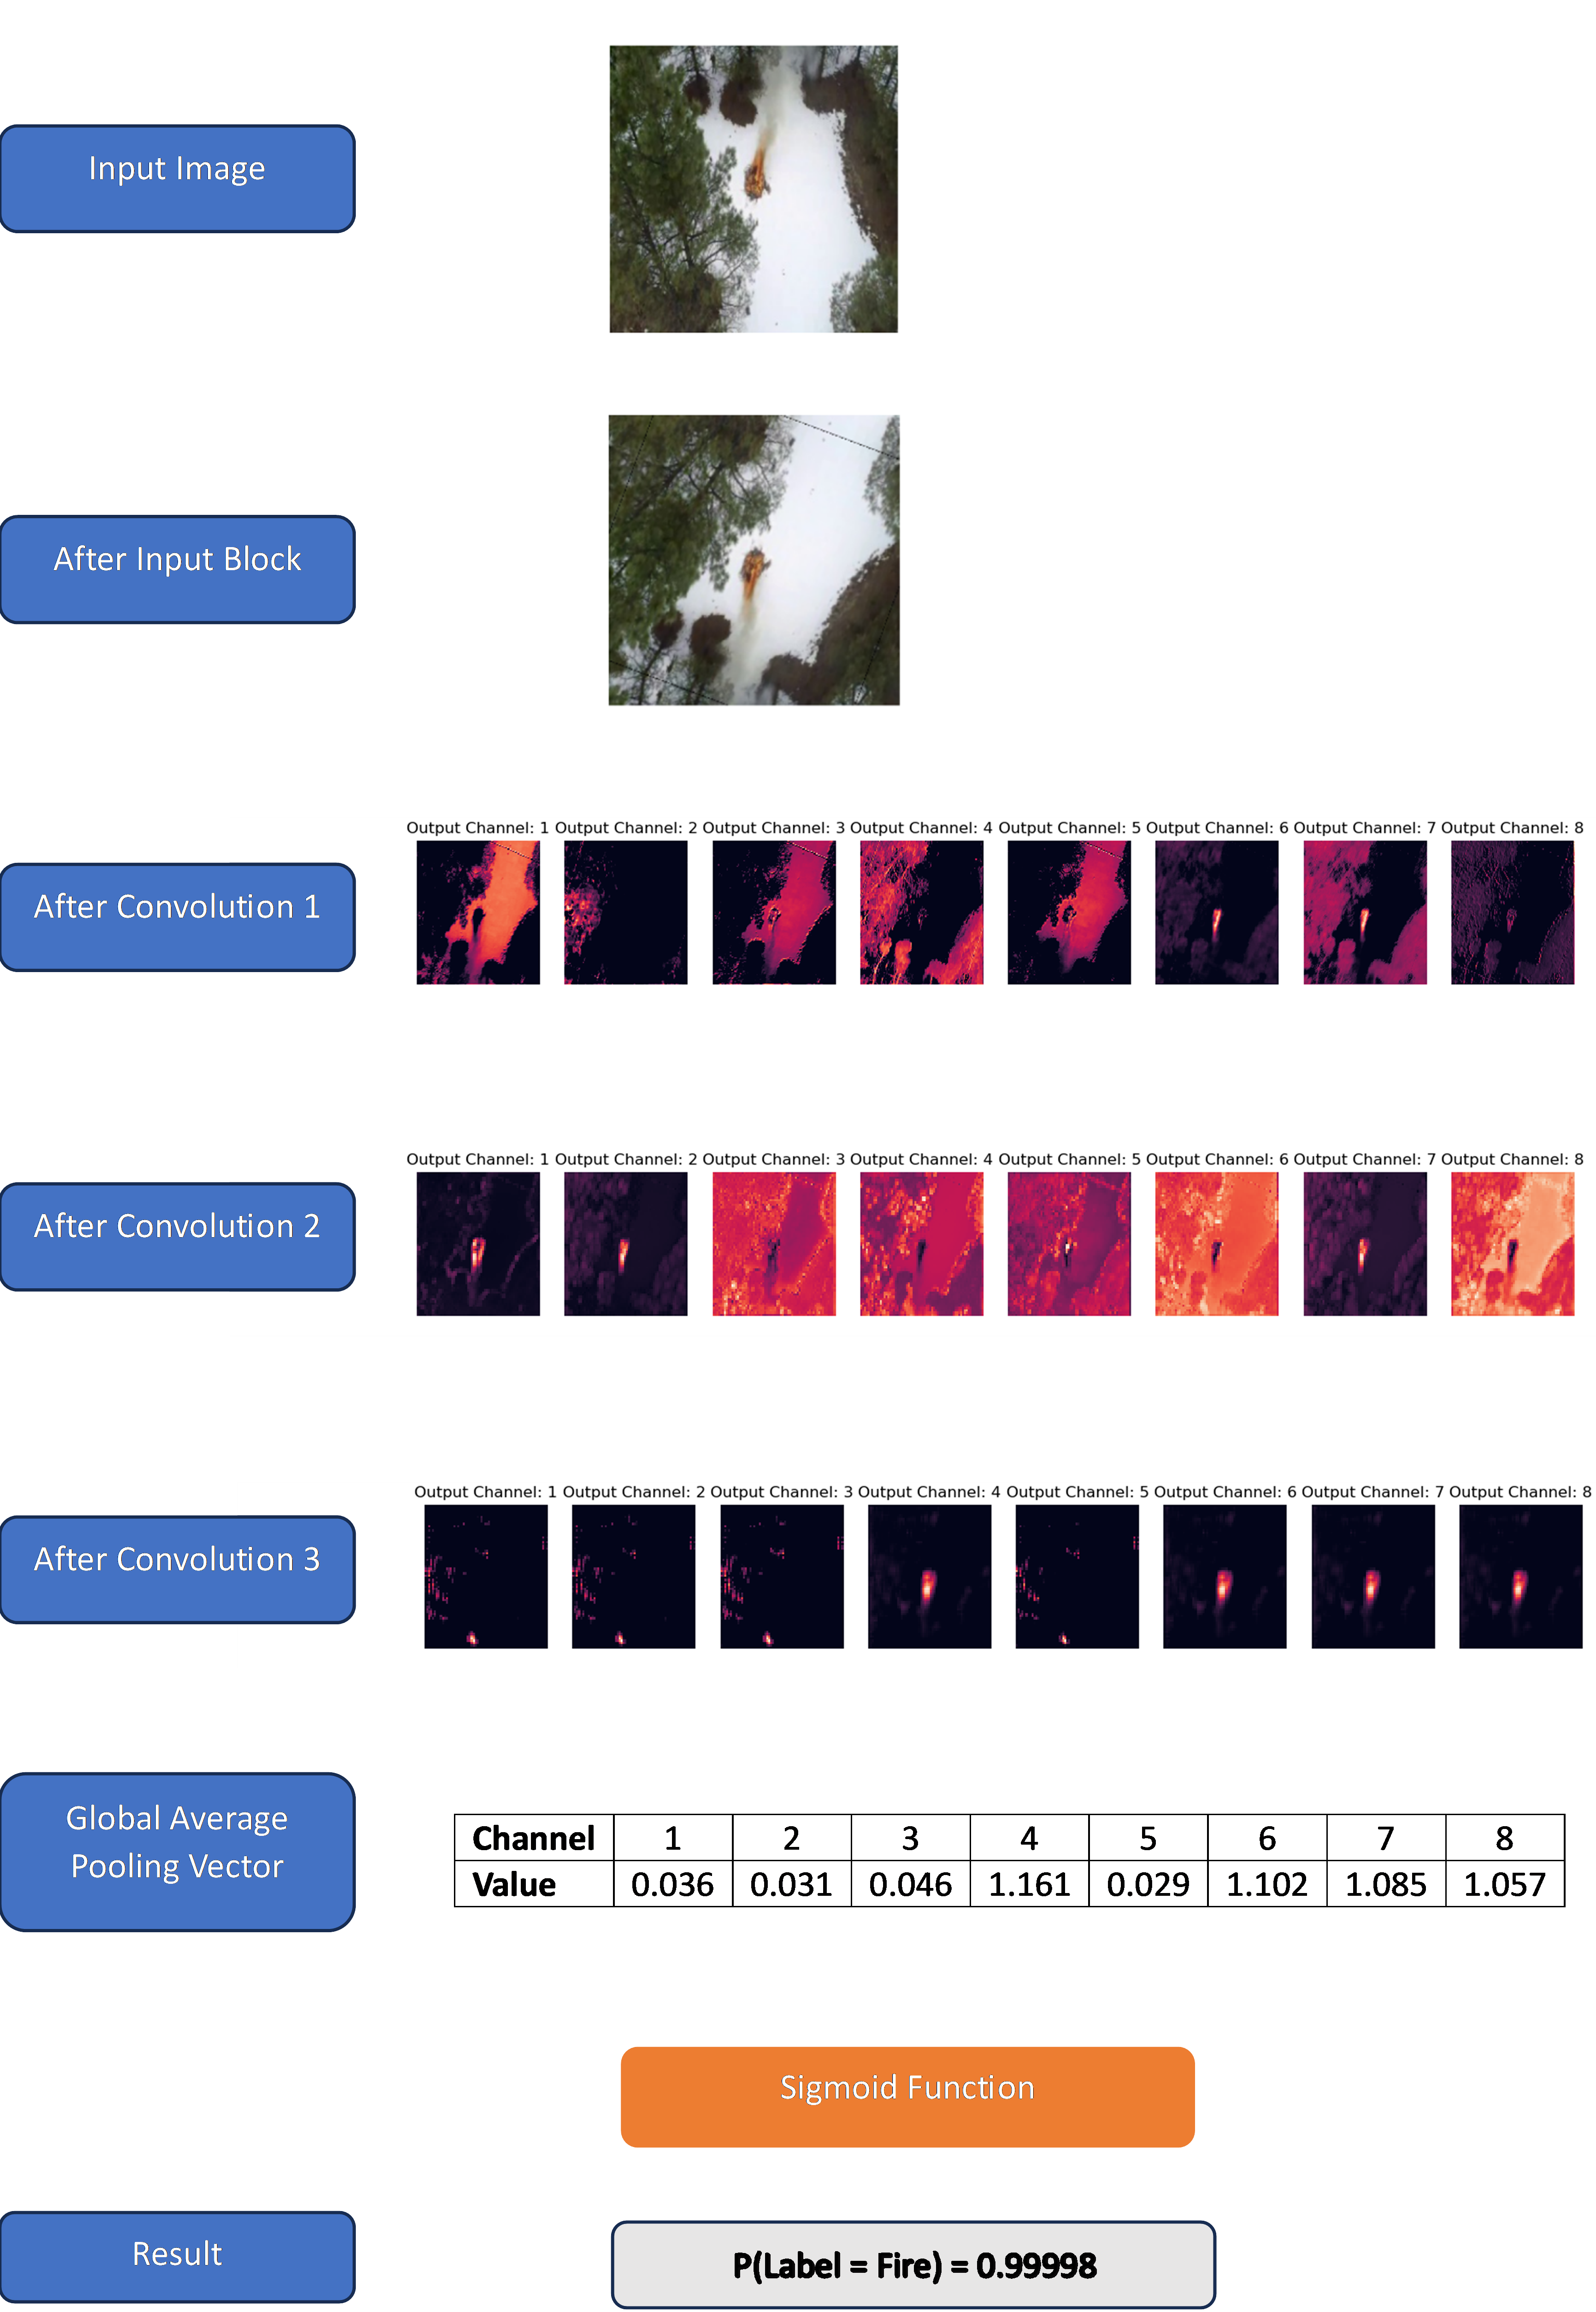
\includegraphics[width=0.9\textwidth]{../figures/model_layers_example/model_layers.png}
    \caption{Model layer convolutions applied to an example image}
\end{figure}


\subsection{Training and Validation Results}
As in \cite{FLAME_dataset}, the model was written using the \verb!tensorflow! Python package, and
was trained with the objective of minimizing the \emph{binary cross-entropy} loss function, which is
suited for binary classification:

\[
    \mathcal{L}(y,\hat{y}) = -\frac{1}{N} \sum_{i=1}^{N} y_i \log (p(\hat{y}_i)) + (1 - y_i) \log (1- p(\hat{y}_i))    
\]

The Adam optimizer is used to minimize the loss function and find the optimal model weights. Please see the DCNN Model training section
in \verb!scripts/UDA_FinalProject_Batek.ipynb! for the training implementation. The code is compatible with
Python version 3.7.12, Tensorflow version 2.3 and Keras version 2.4. For a full list of dependancies, I have exported
a requirements.txt, environment.yml and spec-file.txt to the root of the Github Repositry \cite{Batek_Unstructured_Data_Analysis}.
As I currently do not have access to any computational resources besides my Microsoft Surface Laptop 4, training was computed via
CPU only. Due to this limitation, I reduced the number of epochs for training to 20, as opposed to 40 in \cite{FLAME_dataset}. The training
procedure took approximately 5 hours and 35 minutes to complete using all of the images in the classification Training folder (item 7 in the IEEE Dataport). 

\begin{figure}[h]
    \centering
    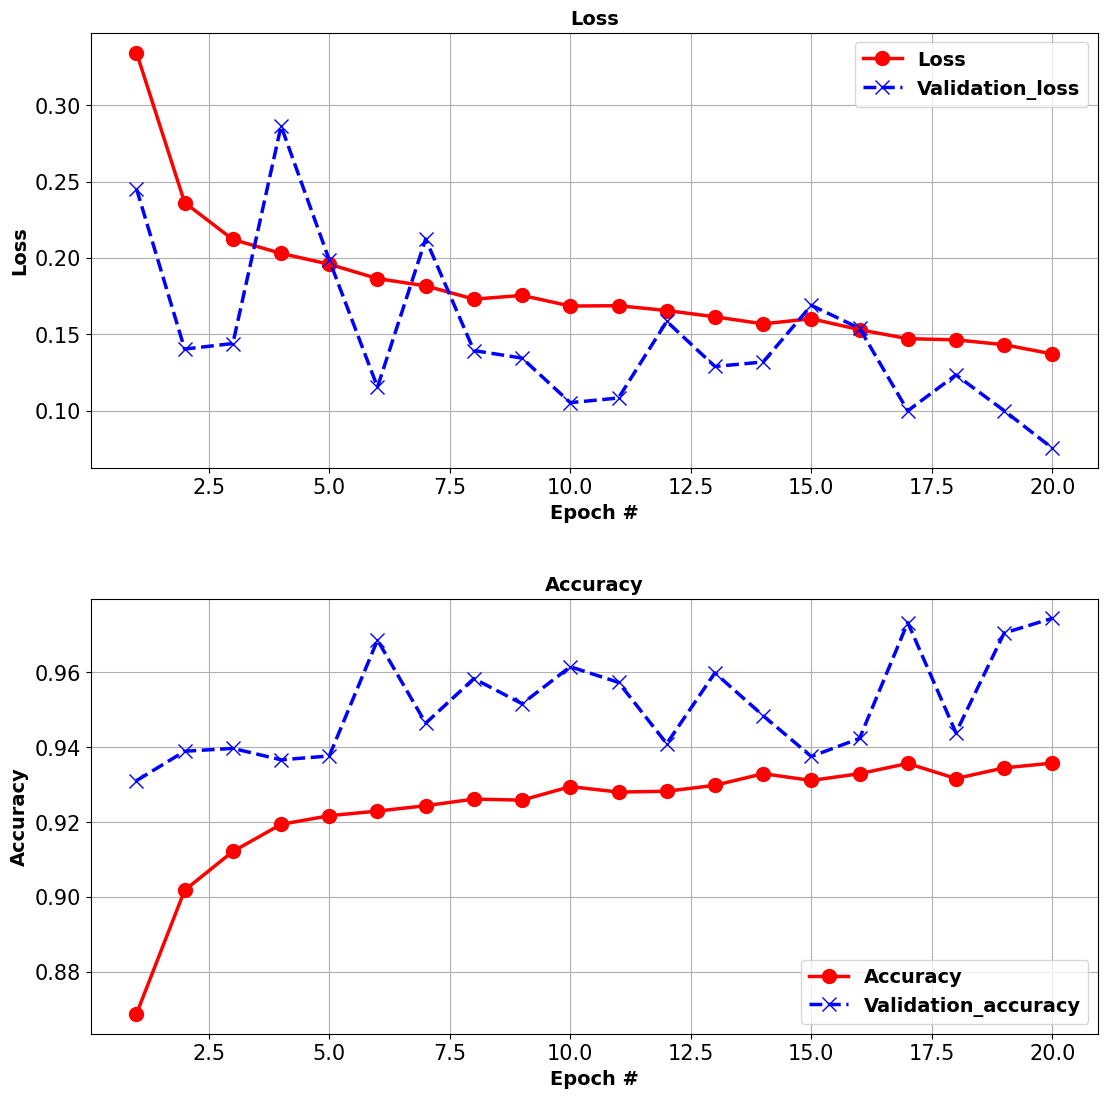
\includegraphics[width=\textwidth]{../figures/training_loss_accuracy.png}
    \caption{Loss and Accuracy during training and against 15\% holdout validation}
\end{figure}

\begin{figure}[h]
    \centering
    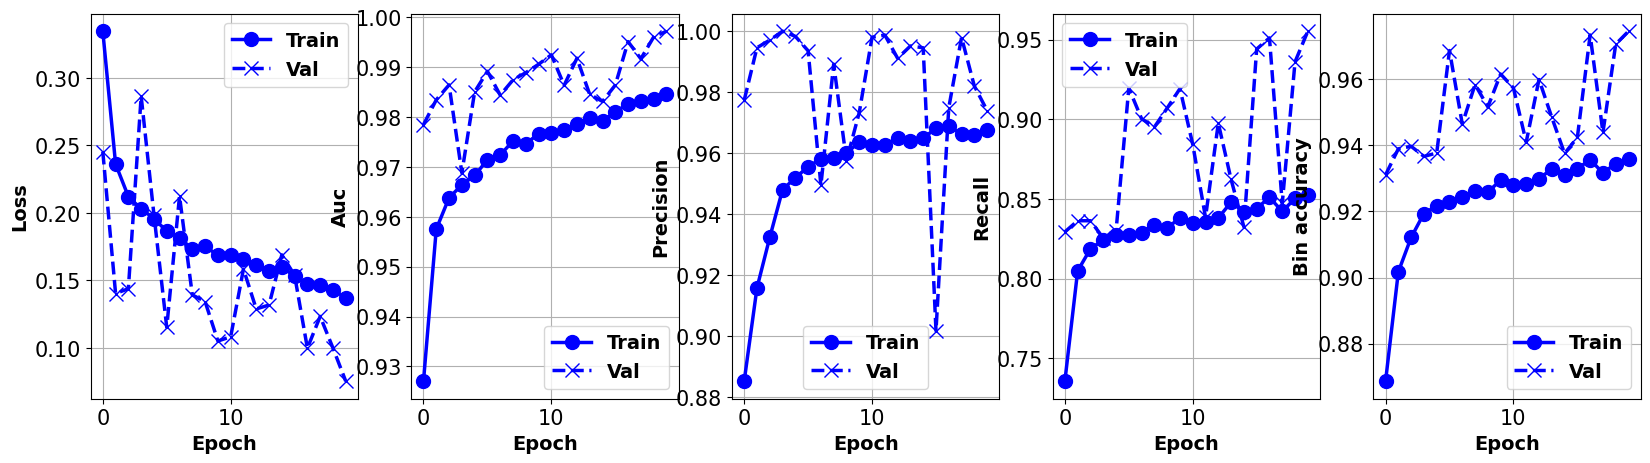
\includegraphics[width=\textwidth]{../figures/training_metrics.png}
    \caption{Accuracy, AUC, Precision, Recall, Binary Accuracy for Training and vs Validation}
\end{figure}

\medskip

Figure 6 shows the training results in terms of Training and Validation loss and accuracy per epoch.
For both Binary Cross Entropy Loss and Binary Accuracy, we see a realitively steady improvement for
each subsequent epoch, in training as well as the validation hold-out comparisons. This shows little
to no evidence of model overfitting, as that would be indicated by a decrease in training loss conciding
with an increase in validation loss (and vice versa for accuracy). Figure 7 reveals the same trend in
terms of AUC, Precision and recall.

\subsection{Testing on Unseen Data}
For the next step, I evaluate the model against the FLAME Dataset Classification Test images (item 8). 
Figure 8 shows the result.



\subsection{Testing on Out of Sample Data}
\blindtext

\section{Summary and Conclusion}
\blindtext

\printbibliography

\end{document}